\documentclass{report}
\usepackage[utf8]{vietnam}
\usepackage[left=2cm,right=2cm,top=1cm,bottom=1cm]{geometry}
\usepackage{graphicx}
\usepackage{hyperref}
\usepackage{amsmath}
\hypersetup{
    colorlinks,
    citecolor=black,
    filecolor=black,
    linkcolor=black,
    urlcolor=black
}

\begin{document}

% Giới thiệu
\begin{center}
    \LARGE
    \textbf{TRƯỜNG ĐẠI HỌC CÔNG NGHỆ}

    \vspace{0.5cm}
    \Large
    \textbf{VIỆN TRÍ TUỆ NHÂN TẠO}

    \vspace{0.5cm}
    \Large
    \textbf{-----***-----}

    \vspace{2.5cm}
    \textbf{BÁO CÁO MÔN HỌC}\\
    \textbf{KỸ THUẬT VÀ CÔNG NGHỆ DỮ LIỆU LỚN}

    \vspace{0.5cm}
    \textbf{ĐỀ TÀI}

    \vspace{0.5cm}
    \centerline{\textbf{HỆ THỐNG ĐỀ XUẤT PHIM DỰA TRÊN}}
    \centerline{\textbf{ITEM COLLABORATIVE FILTERING VÀ HADOOP MAPREDUCE}}

    \vspace{2cm}
    \textbf{Nhóm sinh viên thực hiện:} \\

    \vspace{0.2cm}
    \begin{tabular}{p{8cm}lll}
         & 1. & Nguyễn Mạnh Cường - 22022516 \\
         & 2. & Bùi Đức Mạnh - 22022602      \\
         & 3. & Lê Việt Hùng - 22022666      \\
    \end{tabular}

    \vspace{0.5cm}
    \textbf{Giảng viên hướng dẫn:} \\
    \vspace{0.2cm}
    \begin{tabular}{p{6cm}ll}
         & TS. Trần Hồng Việt \\
         & ThS.Ngô Minh Hương \\
    \end{tabular}

    \vfill

    \textbf{HÀ NỘI, 5/2024}


\end{center}

% Mở đầu
\newpage
\begin{center}
    \section*{MỞ ĐẦU}
\end{center}
\addcontentsline{toc}{section}{\textbf{MỞ ĐẦU}}
\begin{flushleft}
    \vspace{1cm}
    Công nghệ Big data đã đạt đến đỉnh cao trong việc thực hiện các chức năng
    của nó. Trong tháng 8/2015 Big data đã vượt ra khỏi bảng xếp hạng những
    công nghệ mới nổi Cycle Hype của Gartner và tạo ra một tiếng vang lớn cho xu
    hướng công nghệ của thế giới. Big data chứa trong mình rất nhiều thông tin
    quý giá mà nếu mà trích xuất thành công, nó sẽ giúp rất nhiều trong nhiều
    lĩnh vực như y tế, giao thông, giáo dục, …\\
    \vspace{0.5cm}
    Chính vì thế những framework giúp việc xử lý BIGDATA cũng đang ngày càng
    được xử lý và phát triển mạnh. Một trong những công nghệ cốt lõi cho việc
    lưu trữ và truy cập số lượng lớn dữ liệu là Hadoop - một framework giúp lưu
    trữ và xử lý Big data áp dụng MapReduce.\\
    \vspace{0.5cm}
    Từ đó, chúng em đã chọn đề tài: " \textbf{Hệ thống đề xuất phim dựa trên Item
        Collaborative Filtering và Hadoop Mapreduce} " để làm báo kết thúc môn học
    của mình.\\
    \vspace{0.5cm}
    Báo cáo gồm 4 chương
    \begin{itemize}
        \item \textbf{Chương 1}: Tổng quan về dữ liệu lớn
        \item \textbf{Chương 2}: Xây dựng hệ thống gợi ý phim bằng thuật toán
              Item-based Collaborative Filtering
        \item \textbf{Chương 3}: Ứng dụng Hadoop MapReduce với Item-based
              Collaborative Filtering trong Recommendation System
        \item \textbf{Chương 4}: Kết luận và hướng phát triển
    \end{itemize}

\end{flushleft}

% Mục lục
\tableofcontents
\setcounter{page}{2}

% Chapter 1
\chapter[TỔNG QUAN VỀ DỮ LIỆU LỚN]
 {\LARGE TỔNG QUAN VỀ DỮ LIỆU LỚN}

% Section 1 Chapter 1
\section{Định nghĩa}
\begin{flushleft}
    Dữ liệu lớn, hay còn được gọi là Big Data, là thuật ngữ chỉ đến tập hợp dữ
    liệu có kích thước lớn hoặc phức tạp đến mức các phương pháp truyền thống
    không đủ để xử lý. Theo định nghĩa của Wikipedia, dữ liệu lớn là một khái
    niệm chỉ đến các tập dữ liệu có quy mô hoặc độ phức tạp đáng kể, đặc biệt
    là khi các phương pháp truyền thống gặp khó khăn trong việc xử lý chúng.\\
    \vspace{0.5cm}
    Tổ chức nghiên cứu Gartner định nghĩa dữ liệu lớn là những nguồn thông tin
    có đặc điểm chung là kích thước lớn, tốc độ xử lý nhanh và định dạng dữ liệu
    đa dạng. Để khai thác hiệu quả dữ liệu lớn, cần áp dụng các phương pháp và
    công nghệ xử lý mới để thực hiện các quyết định, khám phá thông tin mới và
    tối ưu hóa các quy trình.
\end{flushleft}

% Section 2 Chapter 1
\section{Nguồn hình thành của dữ liệu lớn}
Dữ liệu lớn được tạo thành chủ yếu từ 6 nguồn chính, bao gồm:
\begin{itemize}
    \item \textbf{Dữ liệu hành chính}: Phát sinh từ các hoạt động chương trình của tổ chức,
          bao gồm cả chính phủ và phi chính phủ. Ví dụ như hồ sơ y tế điện tử tại các
          cơ sở y tế, hồ sơ bảo hiểm, thông tin ngân hàng.
    \item \textbf{Dữ liệu thương mại}: Xuất phát từ các giao dịch giữa các thực thể kinh
          doanh. Ví dụ như giao dịch thẻ tín dụng, giao dịch trực tuyến, bao gồm cả các
          giao dịch từ thiết bị di động.
    \item \textbf{Dữ liệu từ cảm biến}: Bao gồm thông tin từ các thiết bị cảm biến như
          máy chụp hình vệ tinh, cảm biến đường, cảm biến khí hậu.
    \item \textbf{Dữ liệu từ thiết bị theo dõi}: Bao gồm thông tin thu thập từ các thiết bị
          theo dõi như điện thoại di động, GPS.
    \item \textbf{Dữ liệu từ hành vi trực tuyến}: Bao gồm thông tin từ các hoạt động trực
          tuyến như tìm kiếm sản phẩm, dịch vụ hoặc thông tin khác, cũng như việc đọc
          các trang web.
    \item \textbf{Dữ liệu từ ý kiến và quan điểm}: Bao gồm thông tin về ý kiến, quan điểm
          của cá nhân hoặc tổ chức trên các nền tảng mạng xã hội và các phương tiện
          truyền thông khác.
\end{itemize}
\begin{figure}[h]
    \centering
    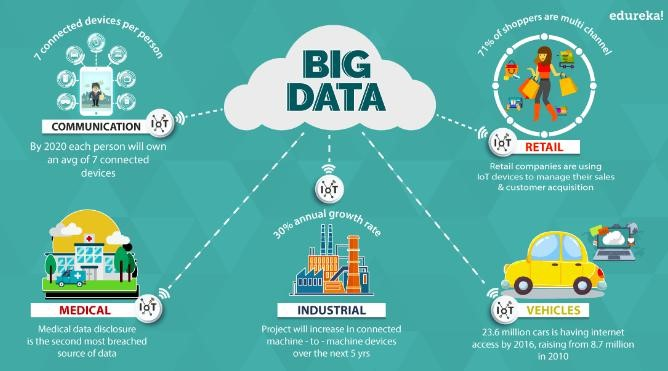
\includegraphics[width=8cm]{images/BigData.jpg}
    \caption{Minh họa nguồn gốc của dữ liệu}
\end{figure}

%Section 3 Chapter 1
\section{Đặc trưng 5V của dữ liệu lớn}
Dữ liệu lớn có 5 đặc điểm cơ bản, được mô hình hóa qua mô hình 5V:
\begin{itemize}
    \item \textbf{Volume (Khối lượng)}: Dữ liệu lớn thường có khối lượng lớn,
          từ hàng terabyte đến petabyte. Để lưu trữ dữ liệu này, chúng ta phải
          sử dụng các công nghệ đám mây mới.
    \item \textbf{Velocity (Tốc độ)}: Dữ liệu lớn được tạo ra và truy cập với
          tốc độ cực kỳ nhanh, đôi khi trong thời gian thực. Điều này đặc biệt quan
          trọng trong các lĩnh vực như Internet, Tài chính, Y tế.
    \item \textbf{Variety (Đa dạng)}: Dữ liệu lớn không chỉ là dữ liệu có cấu trúc
          mà còn bao gồm các loại dữ liệu phi cấu trúc như tài liệu văn bản, hình ảnh,
          video, dữ liệu từ cảm biến vật lý. Việc phân tích và liên kết các loại dữ liệu
          này là thách thức lớn.
    \item \textbf{Veracity (Độ tin cậy/Chính xác)}: DMột trong những vấn đề phức tạp
          nhất của dữ liệu lớn là độ tin cậy và chính xác của dữ liệu. Với sự phát triển
          mạnh mẽ của phương tiện truyền thông xã hội và mạng xã hội, việc đảm bảo tính
          chính xác của dữ liệu trở nên khó khăn hơn.
    \item \textbf{Value (Giá trị)}: Giá trị là yếu tố quan trọng nhất của dữ liệu
          lớn. Trước khi đầu tư vào dữ liệu lớn, chúng ta cần xác định rõ giá trị mà
          thông tin có thể mang lại. Dự báo chính xác và ứng dụng hiệu quả dữ liệu lớn
          có thể mang lại lợi ích lớn, giảm chi phí và tăng hiệu suất trong nhiều lĩnh
          vực.
\end{itemize}

% Section 4 Chapter 1
\section{Tổng quan về Hadoop}
Hadoop là một framework nguồn mở của Apache, viết bằng Java, cho phép
phát triển các ứng dụng phân tán xử lý dữ liệu lớn miễn phí. Nó được
thiết kế để mở rộng từ một máy chủ đơn sang hàng ngàn máy tính khác có
tính toán và lưu trữ cục bộ.
\begin{figure}[h]
    \centering
    
\includegraphics[width=8cm]{images/Hadoop1.jpg}
    \caption{Biểu tượng của Hadoop}
\end{figure}
\newline
Hadoop có cấu trúc liên kết master-slave, với một node master và nhiều
node slave. Node master gán tác vụ và quản lý tài nguyên, trong khi node slave
lưu trữ dữ liệu thực. Hadoop gồm ba lớp chính:
\begin{itemize}
    \item \textbf{HDFS (Hadoop Distributed File System)}: Hệ thống file phân tán
          của Hadoop, cung cấp khả năng lưu trữ dữ liệu lớn trên nhiều node.
    \item \textbf{MapReduce}: Mô hình lập trình và xử lý dữ liệu song song
          của Hadoop.
    \item \textbf{YARN (Yet Another Resource Negotiator)}: Một hệ thống quản lý
          tài nguyên trong Hadoop.
\end{itemize}
\begin{figure}[h]
    \centering
    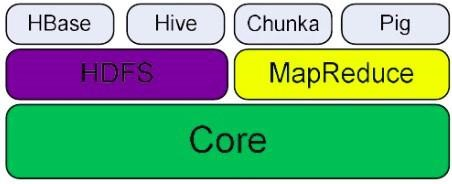
\includegraphics[width=8cm]{images/Hadoop2.jpg}
    \caption{Thành phần của Hadoop}
\end{figure}

% Section 5 Chapter 1
\pagebreak
\section{Tổng quan về MapReduce}
MapReduce là một framework dùng để viết các ứng dụng xử lý song song
một lượng lớn dữ liệu có khả năng chịu lỗi cao xuyên suốt hàng ngàn
cluster (cụm) máy tính.
\vspace{0.5cm}
\newline
MapReduce thực hiện 2 chức năng chính đó là:
\begin{itemize}
    \item \textbf{Map}: Sẽ thực hiện đầu tiên, có chức năng tải,
          phân tích dữ liệu đầu vào và chuyển đổi thành tập
          dữ liệu theo cặp key/value.
    \item \textbf{Reduce}: Sẽ nhận kết quả đầu ra từ tác vụ Map,
          kết hợp dữ liệu lại với nhau thành tập dữ liệu nhỏ hơn, tạo ra
          kết quả cuối cùng.
\end{itemize}
\begin{figure}[h]
    \centering
    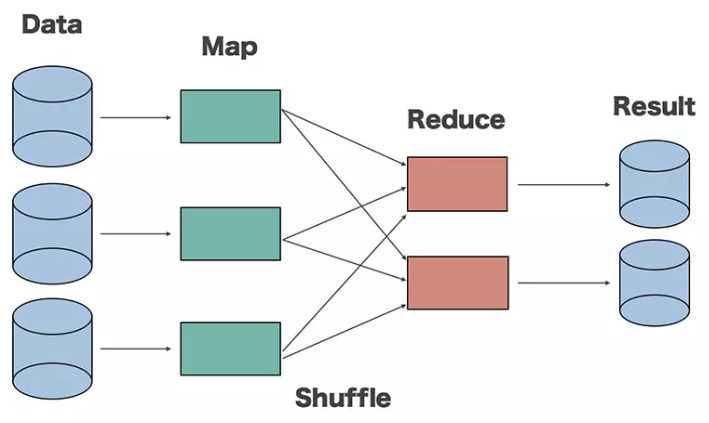
\includegraphics[width=10cm]{images/MapReduce.png}
    \caption{MapReduce}
\end{figure}

% Chapter 2
\chapter[XÂY DỰNG HỆ THỐNG GỢI Ý PHIM BẰNG THUẬT TOÁN ITEM-BASED COLLABORATIVE FILTERING]
 {\LARGE XÂY DỰNG HỆ THỐNG GỢI Ý PHIM BẰNG THUẬT TOÁN ITEM-BASED COLLABORATIVE FILTERING}

% Section 1 Chapter 2
\section{Giới thiệu thuật toán}
Thuật toán Item - based Collaborative Filtering (CF) là một phương pháp
phổ biến trong hệ thống gợi ý, được sử dụng để đưa ra các đề xuất cá nhân
hóa cho người dùng.
\vspace{0.5cm}
\newline
Thuật toán này phân tích ma trận người dùng - sản phẩm
để xác định mối quan hệ giữa các sản phẩm khác nhau và sau đó sử dụng các
mối quan hệ này để tính toán gián tiếp các đề xuất cho người dùng.
\vspace{0.5cm}
\newline
Phương pháp này giúp cải thiện hiệu quả và chất lượng của hệ thống
gợi ý so với các thuật toán CF dựa trên người dùng.

% Section 2 Chapter 2
\section{Triển khai thuật toán}
Triển khai thuật toán Item - based Collaborative Filtering
bao gồm các bước chính sau đây:

\subsection*{Bước 1: Xây dựng ma trận đồng xuất hiện}
Tạo ra ma trận đồng xuất hiện C kích thước n x n, trong đó
C[i][j] là số lượng người dùng đã đánh giá cả sản phẩm i và j.

\subsection*{Bước 2: Chuẩn hóa ma trận}
Tạo ra ma trận chuẩn hóa S kích thước n x n, trong đó: \\
$$S[i][j] = \frac{C[i][j]}{\sum_{m \in M}C[m][j]}$$ \\
Trong đó M là tập hợp tất cả các sản phẩm.

\subsection*{Bước 3: Xây dựng ma trận đánh giá}
Tạo ra ma trận đánh giá R kích thước n x m, trong đó: \\
$$R[i][j] = \sum_{m \in M}S[i][m] \times U[m][j]$$ \\
Trong đó M là tập hợp tất cả các sản phẩm và thay $U[i][j]=?$ thành $U[i][j]=0$

\subsection*{Bước 4: Triển khai với Hadoop MapReduce}
Để triển khai thuật toán này trên một tập dữ liệu lớn, chúng ta sử dụng
Hadoop MapReduce để phân chia và xử lý dữ liệu song song. Quá trình triển khai
bao gồm các bước sau:
\begin{itemize}
    \item \textbf{Mapper}: Đọc vào các cặp key/value biểu diễn dữ liệu
          người dùng - sản phẩm, tính toán các cặp sản phẩm tương tự và
          lưu trữ các kết quả trung gian.
    \item \textbf{Reducer}: Tập hợp các kết quả từ Mapper, tính toán
          độ tương đồng giữa các sản phẩm và tổng hợp các dự đoán cuối cùng.
\end{itemize}

% Section 3 Chapter 2
\raggedright
\section{Ví dụ minh họa thuật toán}
Để minh họa cho quá trình hoạt động của thuật toán CF dựa trên Item,
chúng ta xem xét một ví dụ đơn giản:\\
\vspace{0.5cm}
\textbf{Dữ liệu đầu vào}: Ma trận người dùng -
sản phẩm với các đánh giá từ 1 - 5. (? là sản phẩm mà người dùng đó chưa đánh giá)\\
\renewcommand{\arraystretch}{2}
{\centering
    \begin{tabular}{ |c|c|c|c|c| }
        \hline
                     & Sản phẩm 1 & Sản phẩm 2 & Sản phẩm 3 & Sản phẩm 4 \\
        \hline
        Người dùng A & 5          & 3          & ?          & 4          \\
        \hline
        Người dùng B & 3          & ?          & 2          & 3          \\
        \hline
        Người dùng C & 4          & ?          & 4          & ?          \\
        \hline
        Người dùng D & ?          & 3          & ?          & 5          \\
        \hline
        Người dùng E & ?          & ?          & ?          & ?          \\
        \hline
    \end{tabular}
    \par}

\subsection*{Bước 1: Xây dựng ma trận đồng xuất hiện}
Dựa trên dữ liệu đầu vào, chúng ta xây dựng ma trận đồng xuất hiện C như sau:
(Ví dụ ta thấy rằng có 2 người cùng đánh giá sản phẩm 1 và 3 là Người dùng B và C
nên $C[1][3] = C[3][1] = 2$)\\
\vspace{0.2cm}
{\centering
    \begin{tabular}{ |c|c|c|c|c| }
        \hline
                   & Sản phẩm 1 & Sản phẩm 2 & Sản phẩm 3 & Sản phẩm 4 \\
        \hline
        Sản phẩm 1 & 3          & 1          & 2          & 2          \\
        \hline
        Sản phẩm 2 & 1          & 2          & 0          & 2          \\
        \hline
        Sản phẩm 3 & 2          & 0          & 2          & 1          \\
        \hline
        Sản phẩm 4 & 2          & 2          & 1          & 3          \\
        \hline
    \end{tabular}
    \par}

\subsection*{Bước 2: Chuẩn hóa ma trận}
Dựa trên ma trận C, chúng ta chuẩn hóa thành ma trận S như sau:
(Tổng cột sản phẩm 1 là 8 nên $S[1][1] = \frac{C[1][1]}{8} = \frac{3}{8} = 0.375$)\\
\vspace{0.2cm}
{\centering
    \begin{tabular}{ |c|c|c|c|c| }
        \hline
                   & Sản phẩm 1 & Sản phẩm 2 & Sản phẩm 3 & Sản phẩm 4 \\
        \hline
        Sản phẩm 1 & 0.375      & 0.2        & 0.4        & 0.25       \\
        \hline
        Sản phẩm 2 & 0.125      & 0.4        & 0          & 0.25       \\
        \hline
        Sản phẩm 3 & 0.25       & 0          & 0.4        & 0.125      \\
        \hline
        Sản phẩm 4 & 0.25       & 0.4        & 0.2        & 0.375      \\
        \hline
    \end{tabular}
    \par}

\subsection*{Bước 3: Xây dựng ma trận đánh giá}
Dựa trên ma trận S và ma trận đầu vào U, ta tính được ma trận R như sau:
(Ví dụ ta tính đánh giá của người dùng A cho sản phẩm 3 là
$R[1][3] = 5 \times 0.4 + 3 \times 0 + 0 \times 0.4 + 4 \times 0.2 = 2.8$)\\
{\centering
\begin{tabular}{ |c|c|c|c|c| }
    \hline
                 & Sản phẩm 1 & Sản phẩm 2 & Sản phẩm 3 & Sản phẩm 4 \\
    \hline
    Người dùng A & 3.25       & 3.8        & 2.8        & 3.5        \\
    \hline
    Người dùng B & 2.375      & 1.8        & 2.6        & 2.125      \\
    \hline
    Người dùng C & 2.5        & 0.8        & 3.2        & 1.5        \\
    \hline
    Người dùng D & 1.625      & 3.2        & 1.0        & 2.625      \\
    \hline
    Người dùng E & ?          & ?          & ?          & ?          \\
    \hline
\end{tabular}
\par}
\vspace{0.2cm}
Người dùng E chưa đánh giá sản phẩm nào nên ta không thể tính được đánh giá của người đó.

\subsection*{Kết luận}
Dựa trên tính toán ở trên, dự đoán đánh giá của người dùng A cho Sản phẩm 3 là khoảng 2.8.
Qua ví dụ minh họa này, chúng ta thấy rằng:
\begin{itemize}
    \item Thuật toán CF dựa trên Item giúp xác định mối quan hệ
          giữa các sản phẩm dựa trên đánh giá của người dùng.
    \item Việc tính toán độ tương đồng giữa các sản phẩm và sau đó
          sử dụng nó để tính toán dự đoán đánh giá giúp cải thiện chất lượng gợi ý.
    \item Thuật toán này có thể mở rộng để xử lý dữ liệu lớn bằng cách
          sử dụng Hadoop MapReduce, giúp phân chia và xử lý dữ liệu song song,
          tối ưu hóa hiệu suất và tốc độ xử lý.
\end{itemize}

% Chapter 3
\chapter[ỨNG DỤNG HADOOP MAPREDUCE VỚI ITEM-BASED COLLABORATIVE FILTERING TRONG RECOMMENDATION SYSTEM]
 {\LARGE ỨNG DỤNG HADOOP MAPREDUCE VỚI ITEM-BASED COLLABORATIVE FILTERING TRONG RECOMMENDATION SYSTEM}

% Section 1 Chapter 3
\section{Ý tưởng MapReduce Item-based Collaborative Filtering}
\textbf{Nhiệm vụ}: MapReduce chia quá trình tính toán thành các bước nhỏ hơn \\
\hspace*{2cm}(Map và Reduce), cho phép xử lý song song dữ liệu lớn. \\
\vspace{0.5cm}
\textbf{Ý tưởng}: Phân tán việc tính toán ma trận đồng xuất hiện và ma trận đánh \\
\hspace*{1.7cm}giá qua nhiều máy tính \\
\hspace*{1.7cm}$\rightarrow$ giảm thời gian xử lý và tăng hiệu suất \\
\hspace*{1.7cm}$\rightarrow$ giải quyết các thách thức về kích thước dữ liệu và độ phức tạp của tính toán trong hệ thống gợi ý

% Section 2 Chapter 3
\section{Lưu đồ của thuật toán MapReduce Item-based Collaborative Filtering}
\begin{figure}[h]
    \centering
    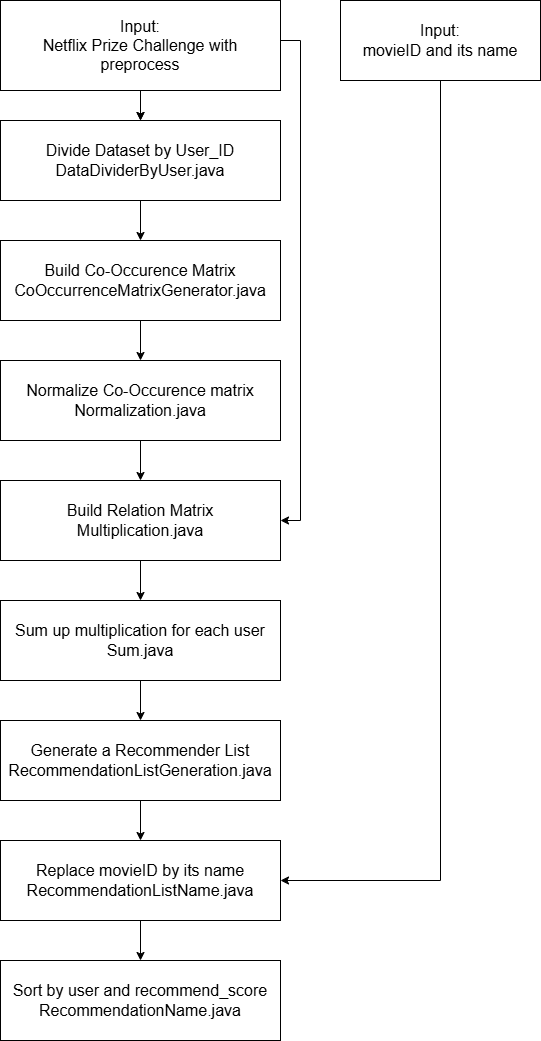
\includegraphics[width=6cm]{images/RecommenderSystem.png}
    \caption{Lưu đồ thuật toán Mapreduce Item-based Collaborative Filtering}
\end{figure}
% Section 3 Chapter 3
\section{Triển khai thuật toán MapReduce Item-based Collaborative Filtering}
\subsection*{Giải pháp Mapreduce cho Item-based Collaborative Filtering}
\begin{itemize}
    \item \textbf{Dữ liệu đầu vào}: Là danh sách các hàng lưu dưới dạng file .txt.
          Mỗi hàng chứa thông tin về người dùng, sản phẩm và đánh giá của người dùng đó
          cho sản phẩm đó, cách nhau bởi dấu phẩy, được chuyển sang kiểu key-value làm
          đầu vào cho thuật toán
    \item \textbf{Triển khai}:
          \begin{enumerate}
              \item Biểu diễn dữ liệu. Dữ liệu lưu trữ dưới dạng list các hàng. Mỗi hàng
                    chứa thông tin về người dùng, sản phẩm và đánh giá của người dùng đó cho
                    sản phẩm đó, cách nhau bởi dấu phẩy.
              \item Lưu trữ phân tán dữ liệu. Dữ liệu được chia thành các phần nhỏ và lưu trữ
                    trên nhiều máy tính khác nhau.
              \item Trên mỗi máy tính, trong mỗi vòng lặp, thực hiện đọc vào từng dòng,
                    gửi lại kết quả cho reducer để tính độ lợi thông tin của từng thuộc tính trong từng phần dữ liệu.
              \item Thực hiện gọi đệ quy xác định nút gốc và nút lá tương ứng.
                    Cập nhật lại nút, cho đến khi đạt hội tụ sau mỗi vòng lặp.\\
                    \vspace{0.2cm}
                    \hspace*{-1cm} $\implies$ \textit{Dữ liệu cần phân lớp}: Là danh sách các hàng lưu trên file .txt. được chuyển sang kiểu key/value làm đầu ra cho thuật toán.
          \end{enumerate}
    \item \textbf{Mô hình cơ bản của MapReduce}:
          \begin{itemize}
              \item Map (KeyIn, ValIn) $\rightarrow$ List(KeyInt, ValInt)
              \item Reduce (KeyInt, List(ValInt)) $\rightarrow$ List(KeyOut, ValOut)
          \end{itemize}
    \item \textbf{Áp dụng cho thuật toán Item-based Collaborative Filtering}:
          \begin{itemize}
              \item Xây dựng lớp DataDividedByUser
              \item Xây dựng lớp CoOccurrenceMatrixGenerator
              \item Xây dựng lớp Normalize
              \item Xây dựng lớp Multiplication
              \item Xây dựng lớp Sum
              \item Xây dựng lớp RecommenderListGenerator
          \end{itemize}
\end{itemize}

\subsection*{Bước 1: Xây dựng lớp DataDividerByUser}
\begin{itemize}
    \item \textbf{Xử lý}: Nhóm dữ liệu theo user \\
    \item \textbf{Mapper}
          \begin{itemize}
              \item \textbf{Input}: user, movie, rating \\
              \item \textbf{Output}: key là user, value là movie:rating \\
          \end{itemize}
    \item \textbf{Reducer}
          \begin{itemize}
              \item \textbf{Input}: key là user, value là movie:rating \\
              \item \textbf{Output}: user \quad movie1:rating1, movie2:rating2, ... \\
          \end{itemize}
\end{itemize}
\subsection*{Bước 2: Xây dựng lớp CoOccurrenceMatrixGenerator}
\begin{itemize}
    \item \textbf{Xử lý}: Đếm số lần mỗi cặp movie được đánh giá bởi cùng 1 người \\
    \item \textbf{Mapper}
          \begin{itemize}
              \item \textbf{Input}: user \quad movie1:rating1, movie2:rating2, ... \\
              \item \textbf{Output}: key là movie1:movie2, value là 1 \\
          \end{itemize}
    \item \textbf{Reducer}
          \begin{itemize}
              \item \textbf{Input}: key là movie1:movie2, value là 1 \\
              \item \textbf{Output}: movie1:movie2 \quad count (trong đó
                    count là số lần cặp movie đó được đánh giá bởi cùng 1 người) \\
          \end{itemize}
\end{itemize}
\subsection*{Bước 3: Xây dựng lớp Normalize}
\begin{itemize}
    \item \textbf{Xử lý}: Chuẩn hóa từng đơn vị của ma trận đồng xuất hiện
          bằng cách chia giá trị đó cho tổng của cột tương ứng trong ma trận
    \item \textbf{Mapper}
          \begin{itemize}
              \item \textbf{Input}: movie1:movie2 \quad count \\
              \item \textbf{Output}: key là movie1, value là movie2:count \\
          \end{itemize}
    \item \textbf{Reducer}
          \begin{itemize}
              \item \textbf{Input}: key là movie1, value là movie2:count \\
              \item \textbf{Output}: movie1 \quad movie2=relation (với relation
                    là giá trị sau khi xử lý) \\
          \end{itemize}
\end{itemize}
\subsection*{Bước 4: Xây dựng lớp Multiplication}
\begin{itemize}
    \item \textbf{Xử lý}: Nhân relation với rating tương ứng với mỗi key là movie
    \item \textbf{CooccurrenceMapper}
          \begin{itemize}
              \item \textbf{Input}: movie1 \quad movie2=relation \\
              \item \textbf{Output}: key là movie1, value là movie2=relation \\
          \end{itemize}
    \item \textbf{RatingMapper}
          \begin{itemize}
              \item \textbf{Input}: user, movie, rating \\
              \item \textbf{Output}: key là movie, value là user:rating \\
          \end{itemize}
    \item \textbf{Reducer}
          \begin{itemize}
              \item \textbf{Input1}: key là movie1, value là movie2=relation \\
              \item \textbf{Input2}: key là movie, value là user:rating \\
              \item \textbf{Output}: user:movie \quad result (với $result = relation \times rating$) \\
          \end{itemize}
\end{itemize}
\subsection*{Bước 5: Xây dựng lớp Sum}
\begin{itemize}
    \item \textbf{Xử lý}: Tính tổng các result theo key là user:movie
    \item \textbf{Mapper}
          \begin{itemize}
              \item \textbf{Input}: user:movie \quad result \\
              \item \textbf{Output}: key là user:movie, value là result \\
          \end{itemize}
    \item \textbf{Reducer}
          \begin{itemize}
              \item \textbf{Input}: key là user:movie, value là result \\
              \item \textbf{Output}: user:movie \quad sum (với sum là tổng các result) \\
          \end{itemize}
\end{itemize}
\subsection*{Bước 6: Xây dựng lớp RecommenderListGenerator}
\begin{itemize}
    \item \textbf{Xử lý}: Lấy ra 5 movie có giá trị sum lớn nhất với mỗi user được sắp xếp giảm dần
    \item \textbf{Mapper}
          \begin{itemize}
              \item \textbf{Input}: user:movie \quad sum \\
              \item \textbf{Output}: key là user, value là movie:sum \\
          \end{itemize}
    \item \textbf{Reducer}
          \begin{itemize}
              \item \textbf{Input}: key là user, value là movie:sum \\
              \item \textbf{Output}: user \quad movie:sum
          \end{itemize}
\end{itemize}

% Section 4 Chapter 3
\section{Demo thuật toán MapReduce Item-based Collaborative Filtering}
\pagebreak
\subsection*{Demo cài đặt hadoop thành công}
\begin{figure}[h]
    \centering
    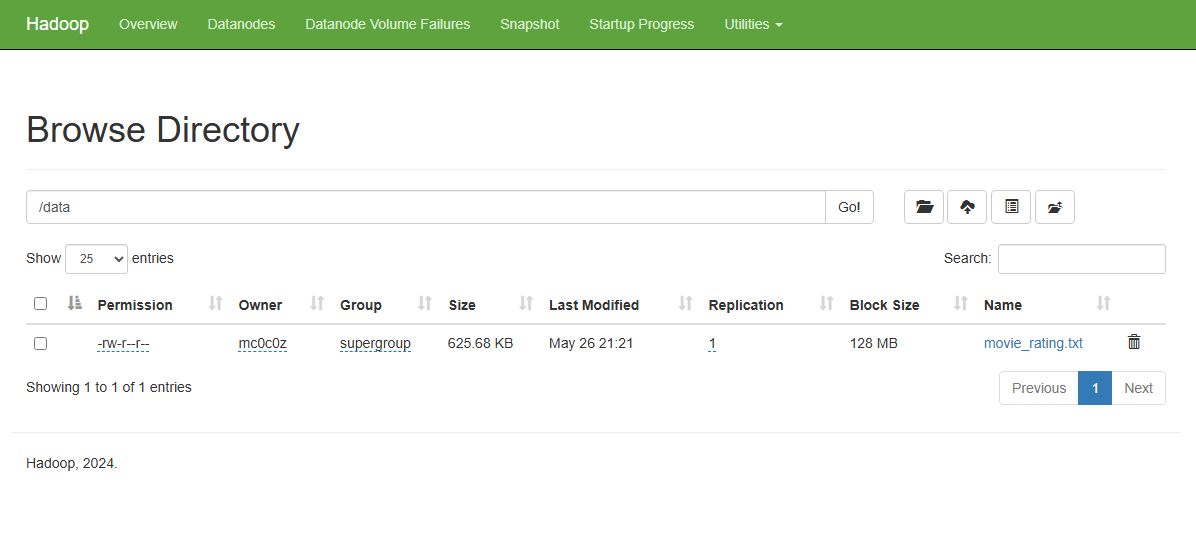
\includegraphics[width=12cm]{images/Demo1.png}
    \caption{Demo cài đặt Hadoop thành công}
\end{figure}
\subsection*{Demo Chương trình}
\begin{enumerate}
    \item Cấu trúc thư mục của Project
          \begin{figure}[h]
              \centering
              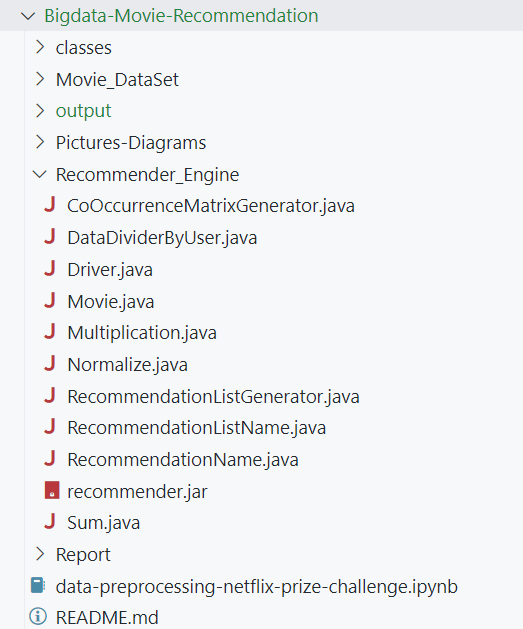
\includegraphics[width=6cm]{images/Demo2.png}
              \caption{Cấu trúc thư mục của Project}
          \end{figure}
    \item Kết quả chương trình
          \begin{figure}[ht]
              \centering
              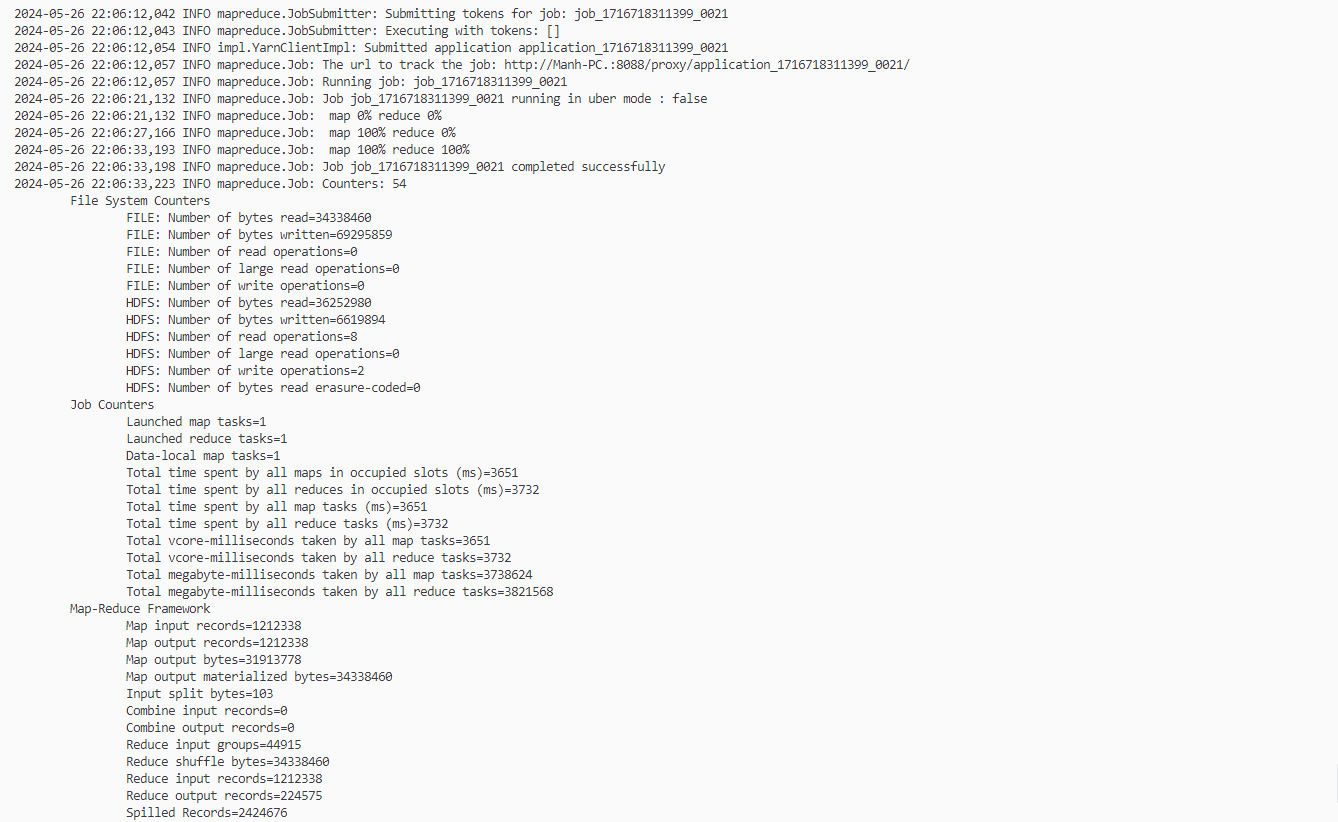
\includegraphics[width=6cm]{images/Demo3.png}
              \caption{Kết quả chương trình}
          \end{figure}
          \pagebreak
    \item File kết quả đầu ra
          \begin{figure}[ht]
              \centering
              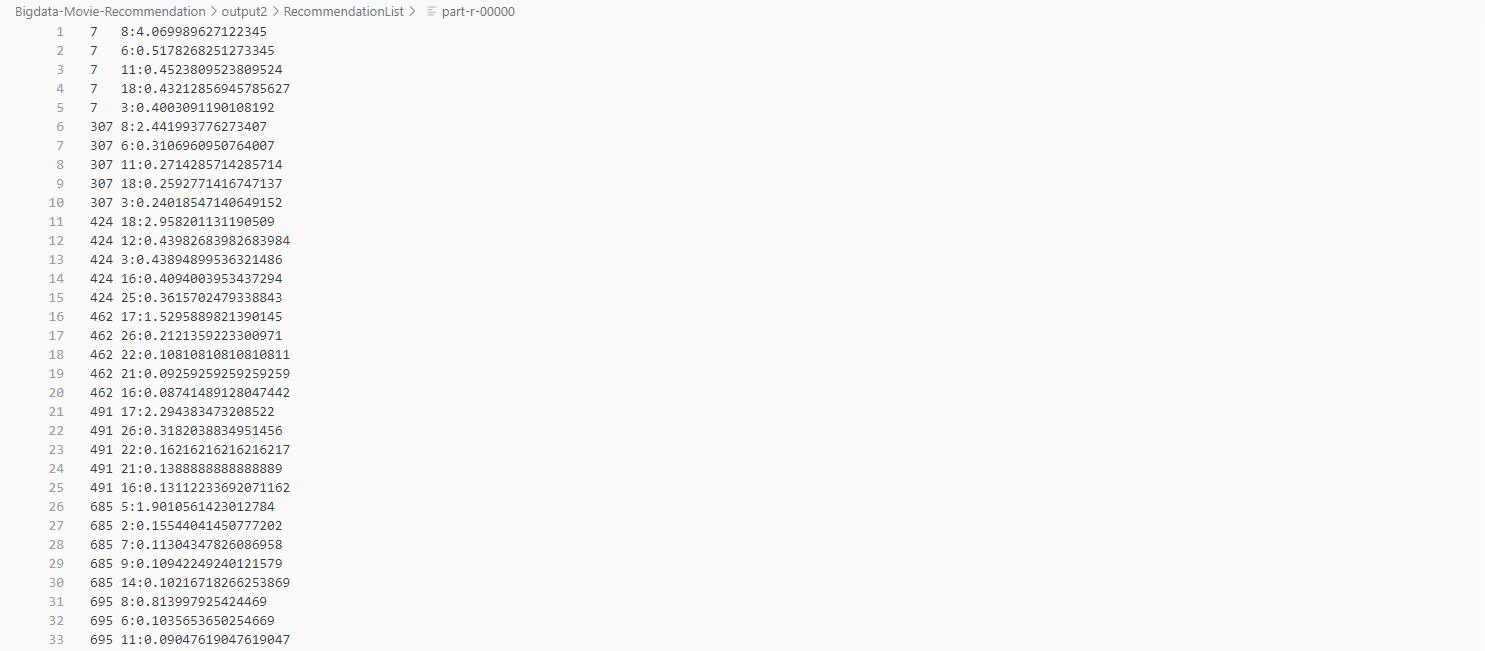
\includegraphics[width=6cm]{images/Demo4.png}
              \caption{File kết quả đầu ra}
          \end{figure}
    \item Đánh giá
          \begin{itemize}
              \item Chương trình đã chạy thành công thuật toán MapReduce Item-based Collaborative Filtering.
              \item Kết quả chạy khớp với kết quả đã thực hiện thủ công trước đó \\ $\rightarrow$ có triển vọng mở rộng với tập dữ liệu lớn hơn
          \end{itemize}
\end{enumerate}


% Chapter 4
\chapter[KẾT LUẬN VÀ HƯỚNG PHÁT TRIỂN]
 {\LARGE KẾT LUẬN VÀ HƯỚNG PHÁT TRIỂN}

% Section 1 Chapter 4
\section{Kết luận}
Big data mang đến cho các tổ chức và doanh nghiệp nhiều cơ hội, thách thức và tài nguyên
giá trị. Mô hình MapReduce giúp giải quyết vấn đề này bằng cách chia công việc xử lý thành
nhiều khối nhỏ, phân tán chúng qua các nút tính toán và sau đó thu thập lại kết quả.
Trong đề tài này, chúng em đã áp dụng mô hình MapReduce trên Hadoop, một framework nguồn mở,
để xây dựng mô hình dự đoán phim dựa trên thuật toán Item-based Collaborative Filtering. \\
\vspace{0.5cm}
Hoàn thành đề tài "Hệ thống đề xuất phim dựa trên Item Collaborative Filtering và Hadoop MapReduce",
nhóm em đã đạt được những kết quả sau:
\begin{itemize}
    \item Hiểu tổng quan về Big Data, Hadoop và MapReduce
    \item Hiểu về thuật toán Item-based Collaborative Filtering
    \item Triển khai ý tưởng và giải pháp cho việc sử dụng Hadoop MapReduce
          trong việc triển khai thuật toán Item-based Collaborative Filtering
    \item Xây dựng lưu đồ thuật toán và triển khai thành công chương trình demo
    \item Đánh giá chương trình.
    \item Do hạn chế về công nghệ nên việc phân tích dữ liệu vẫn còn ở mức nhỏ.
    \item Chương trình demo mới chỉ áp dụng đúng cho dữ liệu đó, dữ liệu khác chưa hỗ trợ được.
\end{itemize}

% Section 2 Chapter 4
\section{Hướng phát triển}
\begin{itemize}
    \item Áp dụng kiến thức về Big data, apache hadoop, cải tiến và xây dựng ứng dụng phân tích
          dữ liệu lớn hơn và vào nhiều lĩnh vực khác.
    \item Trong quá trình hoàn thành bài tập lớn, nhóm em đã cố gắng tìm hiểu và tham khảo các
          tài liệu liên quan. Tuy nhiên, thời gian có hạn nên chúng em sẽ không tránh khỏi những
          thiếu sót, rất mong nhận được sự đóng góp ý kiến của thầy và các bạn để báo cáo và kỹ năng
          của chúng em ngày được hoàn thiện hơn.
\end{itemize}

\begin{center}
    \section*{SẢN PHẨM CỦA NHÓM}
\end{center}
\addcontentsline{toc}{section}{\textbf{SẢN PHẨM CỦA NHÓM}}
\begin{flushleft}
    \vspace{0.5cm}
    \href{https://github.com/manhbd-22022602/Bigdata-Movie-Recommendation}{\textbf{Link GitHub báo cáo của nhóm}}\\
    \vspace{0.5cm}
    \href{https://www.canva.com/design/DAGGDTSDSVg/zqqq_q9GcmJw8djuh1G9Kg/edit}{\textbf{Link Slides thuyết trình của nhóm}}\\
    \vspace{0.5cm}
    \href{https://www.youtube.com/watch?v=rOyGpW_HzME}{\textbf{Link Video demo hệ thống}}
\end{flushleft}

\begin{center}
    \section*{TÀI LIỆU THAM KHẢO}
\end{center}
\addcontentsline{toc}{section}{\textbf{TÀI LIỆU THAM KHẢO}}
\begin{flushleft}
    \vspace{0.5cm}
    \url{https://github.com/thviet79/Bigdata_Project_Recommender_System}\\
    \vspace{0.5cm}
    \url{https://hadoop.apache.org/docs/r1.2.1/mapred_tutorial.html}\\
    \vspace{0.5cm}
    \url{https://www.ra.ethz.ch/cdstore/www10/papers/pdf/p519.pdf}\\
\end{flushleft}

\vfill
\LARGE \centering \textbf{NHIỆM VỤ CỦA CÁC THÀNH VIÊN}
\vspace{0.5cm}
\begin{table}[h!]
    \centering
    \hspace*{-1.2cm}
    \begin{tabular}{|l|p{10cm}|}
        \hline
        \textbf{Sinh viên} & \textbf{Nhiệm vụ}                         \\
        \hline
        Nguyễn Mạnh Cường  &
        \begin{itemize}
            \item Tìm hiểu về Hadoop MapReduce
            \item Tìm hiểu về thuật toán Item-based Collaborative Filtering
            \item Điều hành hoạt động của nhóm
            \item Tham gia viết báo cáo và làm slide
        \end{itemize} \\
        \hline
        Bùi Đức Mạnh       &
        \begin{itemize}
            \item Tìm hiểu về Hadoop MapReduce
            \item Tìm hiểu về thuật toán Item-based Collaborative Filtering
            \item Chỉnh sửa và chạy chương trình
            \item Tham giá viết báo cáo và làm slide
            \item Thuyết trình
        \end{itemize} \\
        \hline
        Lê Việt Hùng       &
        \begin{itemize}
            \item Tìm hiểu về Hadoop MapReduce
            \item Tìm hiểu về thuật toán Item-based Collaborative Filtering
            \item Chỉnh sửa và test code
            \item Tham gia viết báo cáo và làm slide
        \end{itemize} \\
        \hline
    \end{tabular}
    \caption{Bảng công việc}
    \label{tab:my_label}
\end{table}


\end{document}
